% This is a sample LaTeX input file.  (Version of 12 August 2004.)
%
% A '%' character causes TeX to ignore all remaining text on the line,
% and is used for comments like this one.

\documentclass{article}      % Specifies the document class

\def\Course{Statistical Methods for Machine Learning}
\def\Exam{Assignment 2}
\def\Studentname{
Tudor Dragan (xlq880)\\
Nicolae Mariuta (rqt629)\\
Gabriel Carp (slp670)
}
\def\Sub_date{\today}
                             % The preamble begins here.
%\title{\bf Principles of Computer Systems Design\\ {\Large Exam}}  % Declares the document's title.
%\author{Tudor Dragan\\}

\title{\textbf{\Course}\\\textbf{\Exam}}
\author{\Studentname}
\date{\Sub_date}      % Deleting this command produces today's date.

\usepackage{verbatimbox}
\usepackage{listings}
\usepackage{color}
\usepackage[]{amsmath}
\usepackage[english]{babel}
\usepackage[utf8]{inputenc}
\usepackage{graphicx}
\usepackage{moreverb}
\usepackage{hyperref}
\usepackage[T1]{fontenc} % font
\usepackage{program}
\usepackage[top=1.5in, bottom=1.5in, left=1.4in, right=1.4in]{geometry}
\usepackage[super]{nth}
\usepackage{fancyhdr}
\usepackage{lastpage}
\usepackage{float}
\usepackage[section]{placeins}
\usepackage[linesnumbered]{algorithm2e}
\usepackage[table,xcdraw]{xcolor}
\definecolor{dkgreen}{rgb}{0,0.6,0}
\definecolor{gray}{rgb}{0.5,0.5,0.5}
\definecolor{mauve}{rgb}{0.58,0,0.82}
\usepackage[table,xcdraw]{xcolor}
\lhead{\textbf{\Course}}
\rhead{\Exam~(Submission: \Sub_date)}

\cfoot{}
\lfoot{\Studentname}
\rfoot{\thepage\ of \pageref{LastPage}}
%\pagestyle{fancy}
\renewcommand{\footrulewidth}{0.4pt}

\lstset{frame=tb,
      language=Java,
      aboveskip=3mm,
      belowskip=3mm,
      showstringspaces=false,
      columns=flexible,
      basicstyle={\small\ttfamily},
      numbers=none,
      numberstyle=\tiny\color{gray},
      keywordstyle=\color{blue},
      commentstyle=\color{dkgreen},
      stringstyle=\color{mauve},
      breakatwhitespace=true
      tabsize=3
}
\newcommand{\ip}[2]{(#1, #2)}
                             % Defines \ip{arg1}{arg2} to mean
                             % (arg1, arg2).

%\newcommand{\ip}[2]{\langle #1 | #2\rangle}
                             % This is an alternative definition of
                             % \ip that is commented out.

\begin{document}             % End of preamble and beginning of text.

\maketitle                   % Produces the title.

\section*{II.1 Classification}
\subsection*{II.1.1 Linear discriminant analysis}

We have implemented the LDA algorithm according to the slides from the Linear Classification lecture. We also checked with the MATLAB \emph{predict} function from the \emph{ClassificationDiscriminant} class and we have similar results with only a $10^{-3}$ error. As expected the train error is lower than the test error\\

\[ 
train_{ERR} = 0.1500 \]

\[ 
test_{ERR} = 0.2105 
\] \\

\subsection*{II.1.2 Linear discriminant analysis}

We normalized both data sets and applied the LDA algorithm. We noticed that we get the same results as the non-normalized data. This would imply that the normalization has no effect on the accuracy of the LDA classifier. This happens because in \[ \delta_k(x) = x^T\Sigma^{-1}\mu_k - 1/2{\mu_k}^T\Sigma^-1\mu_k + ln{Pr( Y = C_k)}\] the data points are multiplied by the covariance inverse and the mean is subtracted, thus doing a normalization inside the classifier. If we would normalize the data before applying the LDA classifier, the mean is 0 and the covariance is $I$ which would imply that we obtain the same results as we did with the non normalized data set.

\subsection*{II.1.3 Bayes optimal classification and probabilistic classification}

For the given problem, we have thy hypothesis class 
\[H={h0(x)=0, h1(x)=1} \]
 because there it is only one element in the input space and possible values are \emph{0} or \emph{1}. The Bayes optimal classifier is the hypothesis for which we have the minimal risk: min({1 ? 1/4, 1 ? 3/4}) = 1?4 which corresponds to the risk of hypothesis h1(x). The risk of the classifier is the sum of the risks for each classifier. 
\[p(y=0, h(x)=1) = p(y=0 \| h(x)=1)p(h(x)=1) = 0.25 * 0.75 = 0.1875\] 
\[p(y=1, h(x)=0) = p(y=1 \| h(x)=0)p(h(x)=0) = 0.75 * 0.25 = 0.1875\] 
\[Rp(h) = 0.1875 + 0.1875 = 0.375\] 
As a conclusion, the risk of this classifier is worse than using the Bayes optimal classifier.\\
\section*{II.2 Regression: Sunspot Prediction}

\subsection*{II.2.1 Maximum likelihood solution}

We used 3.15 and 3.16 to obtain the construct the design matrixes and train each of these models on the training set by finding the maximum likelihood estimate for the 3 selections. We have plotted for each selection the measured values from the test set and the predicted ones from our algorithm. As we can see from the 3 graphs the best results are obtained from considering all parameters.\\

The RMSs for each selection are: \\
\[ RMS_1 = 35.4651\]
\[ RMS_2 = 28.8398\]
\[ RMS_3 = 18.7700\]


\begin{figure}[ht]
\centering
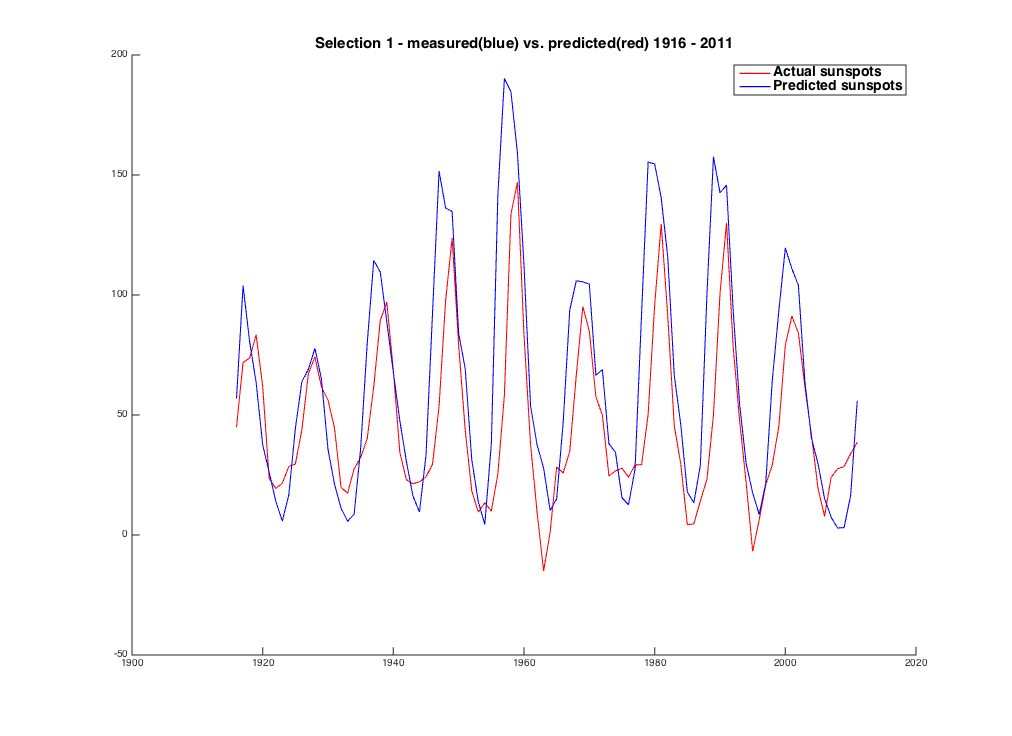
\includegraphics[scale=.4]{img/pred1}
\caption{Selection 1 - measured(blue) vs. predicted(red) 1916 - 2011 \label{overflow}}
\end{figure}

\begin{figure}[ht]
\centering
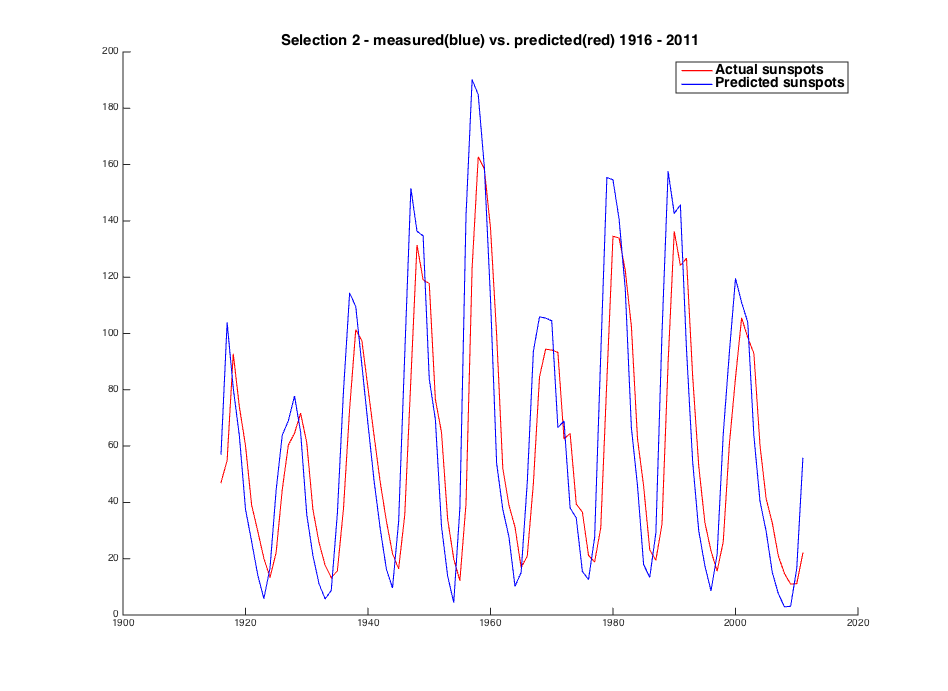
\includegraphics[scale=.4]{img/pred2}
\caption{Selection 3 - measured(blue) vs. predicted(red) 1916 - 2011 \label{overflow}}
\end{figure}

\begin{figure}[ht]
\centering
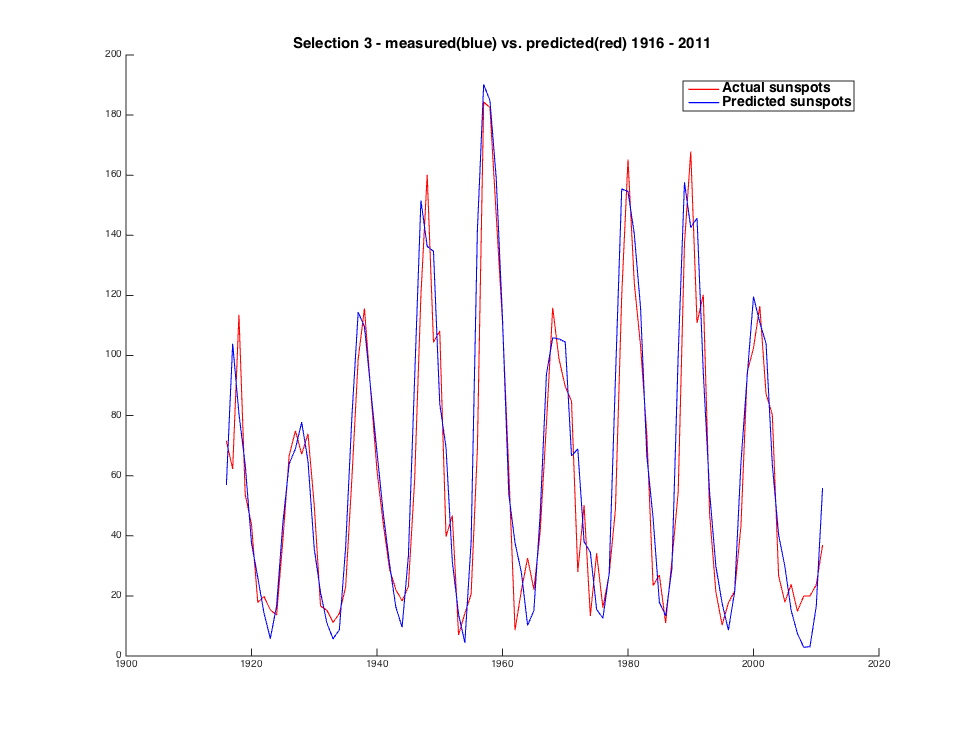
\includegraphics[scale=.4]{img/pred3}
\caption{Selection 3 - measured(blue) vs. predicted(red) 1916 - 2011 \label{overflow}}
\end{figure}

For the $2^{nd}$ selection we have plotted the predicted values shown in Figure 4. Because we have only one set of parameters we have only a $1^{st}$ degree equation which is shown as a straight line. \\

\begin{figure}[ht]
\centering
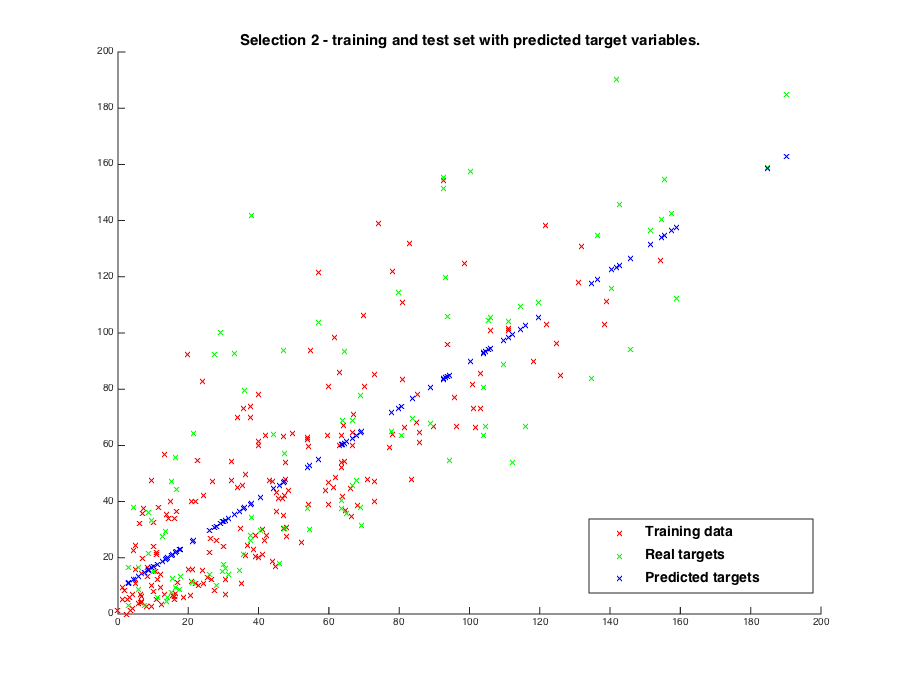
\includegraphics[scale=.4]{img/sel2-pred}
\caption{Predicted values for Selection 2 \label{overflow}}
\end{figure}

\subsection*{II.2.2 Maximum a posteriori solution}

We have implemented the Maximum a posteriori algorithm using (3.52-3.54) equations. We used $\beta = 1$ and we chose $\alpha$ with values between $10^{-10}$ and $10^{10}$. As we can see from Figure 5 with the values of RMS spanned across our alpha interval the best outcome is set by using Selection 3. We will analyze only the $\alpha$ values for selection 3 further. Between $10^{-10}$ and $10^{-2}$ we have the same RMS as the Maximum likelihood solution and for $10^{-1}$ the RMS is lower and the best estimation we get from $\alpha$ set to $10$. Almost the same happens with the other selections, only on different $\alpha$ values.\\

\begin{figure}[ht]
\centering
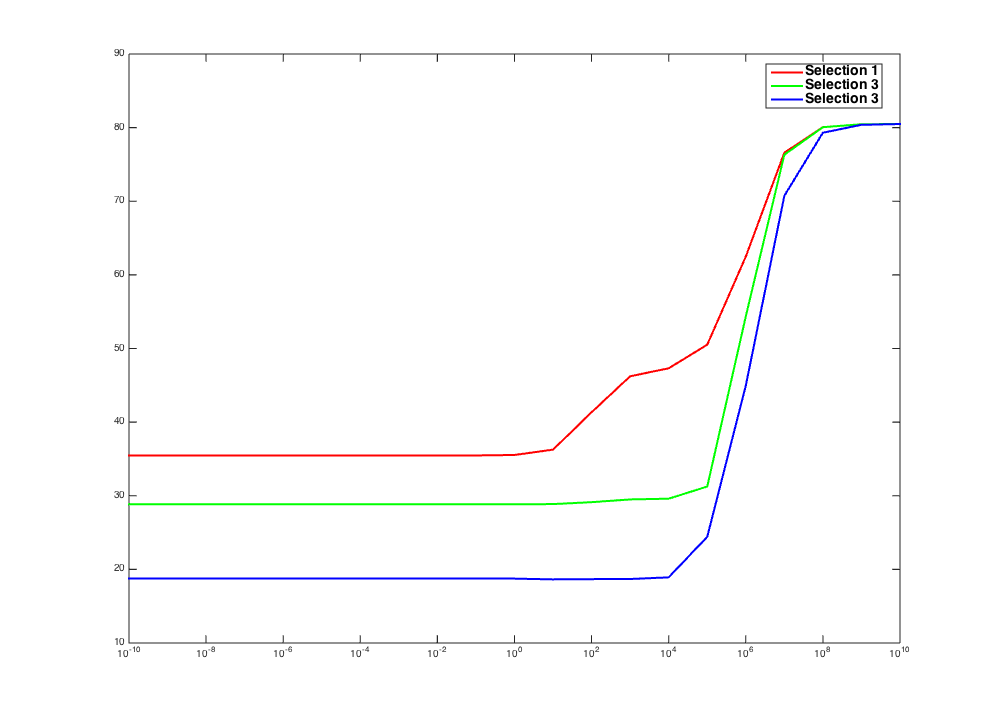
\includegraphics[scale=.4]{img/rms}
\caption{RMS error plotted over alpha values between $10^{-10}$ and $10^{10}$  \label{overflow}}
\end{figure}

\subsection*{II.2.3 Weighted sum-of-squares}

According to Equation 3.11:

\[
log p(t \| w, \beta) = \frac{N}{2}log\beta - \frac{N}{2}log 2\pi - \beta E_D(w) 
\]

we determine the gradient for $E_D(w)$ and equalize it to $0$

\[
\nabla E_D(w) =  \sum_{i=1}^{n} r_n\{t_n - w^T \phi(x_n)\}\phi(x_n)^T
\]

\[
0 =  \sum_{i=1}^{n} r_nt_n\phi(x_n)^T - r_nw^T(\sum_{i=1}^{n} \phi(x_n)^T)
\]

\[
0 = \Phi^TRt - w^T(\Phi^TR\Phi)
\]
,where $R = diag(r_1, r_2, ... r_n)$. Solving it for $w$ we get 

\[
 w = (\Phi^TR\Phi)^{-1}\Phi^TRt
\]

Given the interpretation in terms of 

\begin{description}
   \item [(i) data dependent noise variance]\hfill \\
   We can see that $r_n$ can be considered as an inverse variance vector specific to the data point $(x_n, t_n)$ that can be interpreted as a scaling of $\beta$.
   \item [(ii) replicated data points]\hfill \\
   We can say that $r_n$ can represent an effective number of replicated observations of this specific instance $(x_n, t_n)$ particularly if we restrict $r_n$ to be a positive integer.
\end{description}

\end{document}               % End of document.